%\documentclass[twocolumn,showpacs,preprintnumbers,amsmath,amssymb, floatfix]{revtex4}
\documentclass[aps,prb,preprint,preprintnumbers,amsmath,amssymb,floatfix,superscriptaddress]{revtex4}
%\documentclass[aps,prb,twocolumn,superscriptaddress,preprintnumbers,amsmath,amssymb,floatfix]{revtex4}

\usepackage{graphicx}
\usepackage{epstopdf}
\usepackage{ifthen}
\usepackage{dcolumn}
\usepackage{bm}
\usepackage{multirow}
\usepackage{booktabs}
\usepackage{amsbsy}
\usepackage{amsmath}
\usepackage{amssymb}
\usepackage{subfigure}
\usepackage{booktabs}
\usepackage{verbatim}

\graphicspath{
{/Users/mullspace/Dropbox/git/plots.nogit/images/}
{/home/schuberm/Dropbox/git/plots.nogit/images/}
{/home/mullspace/Dropbox/git/plots.nogit/images/}
}

%--------------------------------------------------------------------------
%DEFINE COMMANDS
%--------------------------------------------------------------------------
\newcommand{\EXP}[1]{\exp\mspace{-5.0mu}\left[#1\right]\mspace{-3.0mu}}

\newcommand{\SUM}[2]{\ifthenelse{\equal{#1}{0}}{\sum_{
\alpha_{#2},b_{#2},l_{#2}}^{3,4L,N}} {\ifthenelse{\equal{#1}{1}}{\sum_{
\alpha_{#2},b_{#2}}^{3,n}}{\sum_{\pmb{\kappa}#2,\nu#2}^{N,3n}}}}

\newcommand{\ab}[2]{\mspace{-4.0mu}\left(\mspace{-8.0mu}
\begin{smallmatrix}&\ifthenelse{\equal{#1}{}}{a}{#1} \\&\ifthenelse
{\equal{#2}{}}{b}{#2}\end{smallmatrix}\mspace{-3.0mu}\right)}

\newcommand{\kvba}{\mspace{-4.0mu}\left(\mspace{-8.0mu}
\begin{smallmatrix} &\pmb{\kappa} &b \\ &\nu &\alpha\end{smallmatrix}
\mspace{-3.0mu}\right)}

\newcommand{\kvbap}{\mspace{-4.0mu}\left(\mspace{-8.0mu}
\begin{smallmatrix} &\pmb{\kappa}' &b \\ &\nu' &\alpha\end{smallmatrix}
\mspace{-3.0mu}\right)}

\newcommand{\kvt}{\mspace{-4.0mu}\left(\mspace{-8.0mu}
\begin{smallmatrix}&\pmb{\kappa} \\&\nu\end{smallmatrix}
\mspace{-2.0mu},t\right)}

\newcommand{\kvw}{\mspace{-4.0mu}\left(\mspace{-8.0mu}
\begin{smallmatrix}&\pmb{\kappa} \\&\nu\end{smallmatrix}
\mspace{-2.0mu},\omega\right)}

\newcommand{\kv}{\mspace{-4.0mu}\left(\mspace{-8.0mu}
\begin{smallmatrix}&\pmb{\kappa} \\&\nu\end{smallmatrix}
\mspace{-3.0mu}\right)}

\newcommand{\kvp}{\mspace{-4.0mu}\left(\mspace{-8.0mu}
\begin{smallmatrix}&\pmb{\kappa'} \\&\nu'\end{smallmatrix}
\mspace{-3.0mu}\right)}

\newcommand{\kw}{\mspace{-4.0mu}\left(\mspace{-8.0mu}
\begin{smallmatrix}&\pmb{\kappa} \\&\omega\end{smallmatrix}
\mspace{-3.0mu}\right)}

\newcommand{\lbt}{\mspace{-4.0mu}\left(\mspace{-8.0mu}
\begin{smallmatrix}&l \\&b\end{smallmatrix}\mspace{-2.0mu},t\right)}
%--------------------------------------------------------------------------
%END COMMANDS
%--------------------------------------------------------------------------
%--------------------------------------------------------------------------
\begin{document}

\title{Disruption of Superlattice Phonons through Interfacial Mixing}
\author{Samuel C. Huberman}
\affiliation{Department of Mechanical \& Industrial Engineering, University of Toronto, 
Toronto, Ontario M5S 3G8, Canada}
\author{Jason M. Larkin}
\affiliation{Department of Mechanical Engineering\\Carnegie Mellon University\\Pittsburgh, PA 15213}
\author{Alan J. H. McGaughey}
%\email{mcgaughey@cmu.edu}
\affiliation{Department of Mechanical Engineering\\Carnegie Mellon University\\Pittsburgh, PA 15213}
\author{Cristina H. Amon}
\affiliation{Department of Mechanical \& Industrial Engineering, University of Toronto, 
Toronto, Ontario M5S 3G8, Canada}
\affiliation{Department of Mechanical Engineering\\Carnegie Mellon University\\Pittsburgh, PA 15213}

\date{\today}% It is always \today, today,
             %  but any date may be explicitly specified
\vspace{14mm}
  
\begin{abstract}

We use normal mode decomposition to obtain phonon properties from quasi-harmonic lattice dynamics calculations and classical molecular dynamics simulations in unstrained Lennard-Jones argon superlattices. The relaxation-time approximation of the Boltzmann transport equation is used to predict cross-plane and in-plane thermal conductivity for a range of superlattice period lengths. Debye scaling ($\omega^{-2}$) of phonon lifetimes is found a low frequencies and Rayleigh scaling ($\omega^{-4}$) for intermediate frequencies in superlattices with interfacial mixing. We find that interspecies mixing reduces a phonon's mean free path and for short-period superlattices, lifetimes below the Ioffe-Regel limit are observed.

\end{abstract}
\maketitle
%%%%
\section{Introduction}

The thermal transport in superlattices, a system that consists typically of periodic alternating films (layers) of dissimilar atoms, has been conventionally studied through molecular dynamics (MD) simulations or Boltzmann Transport Equation (BTE) based methods. MD superlattice studies used the equilibrium  Green-Kubo\cite {PhysRevB.85.195302} technique or the non-equilibrium \cite{PhysRevB.79.214307,PhysRevB.79.075316,PhysRevB.72.174302} direct method to predict cross-plane thermal conductivity. BTE studies relied upon the validity of bulk phonon properties\cite{walkauskas:2579,chen:220} and approximations of the specularity and diffusivity of the interfaces \cite {PhysRevB.57.14958}. While these techniques can make predictions about the trends of thermal conductivity, a mode by mode analysis is required to understand the effects of the secondary periodicity and interfacial mixing upon phonon properties. 

Recent work used Density Functional Perturbation Theory (DFPT) to examine phonon properties in Si/Ge superlattice structures. Garg et al. reported a significant discrepancy between theoretically predicted and experimentally measured cross-plane thermal conductivities which was attributed to the exclusion of mass defect scattering in the DFPT calculation but expected to be present in experimental samples. \cite{doi:10.1021/nl202186y} This conclusion was echoed by Savic et al. using a Monte Carlo approach to the BTE. \cite{savic:073113}. Luckyanova et al. \cite{Luckyanova16112012} adopted Tamura elastic mass defect scattering theory \cite{tamura_isotope_1983} to modify the DFPT predicted lifetimes through the Matthiesen rule.

Mode by mode studies are computationally expensive and limited Broido et al. to a range of period lengths.\cite {PhysRevB.70.081310} For similar reasons, the phonon properties for short period superlattices obtained from DFPT were presumed to hold for larger period superlattices \cite{Luckyanova16112012, doi:10.1021/nl202186y} and the phonon lifetimes of low frequency modes used in the Monte Carlo BTE approach are fitted to a power law. \cite{savic:073113}

In this work, we demonstrate the ability of normal mode decomposition (NMD) to predict the phonon properties in unstrained superlattices with perfect and mixed interfaces without extending phonon properties from short period to large period superlattices. The crucial ingredient is to use the eigenvectors (polarization) vectors of the perfect superlattice to obtain lifetimes in the mixed superlattice. This assumption of perturbative (weak) disorder, where Tamura elastic mass defect scattering theory can be applied, was found to be valid for predicting cross-plane thermal conductivities but not in-plane thermal conductivities in mixed superlattices. 

\section{Modeling Framework}
\subsection{Superlattice structure and interactions}\label{SEC:sl_struc}
%%%
The superlattices are built by placing atoms on a face centered cubic lattice, with the two species only differentiated by their masses. Atomic interactions are modeled using the Lennard-Jones (LJ) potential for argon with an energy scale of $\epsilon= 1.67\times10^{-21}$ Joules, a length scale of $\sigma= 3.4\times10^{-10}$ meters, a mass scale of $m= 6.63\times10^{-26}$ kg and are truncated at a cutoff radius of $2.5\sigma$. The lighter species has a mass $m$ and the heavier species has a mass $3m$. Dimensionless LJ units are used unless otherwise noted. The temperature is fixed at 20 K for which the zero-pressure lattice constant is $a=5.315 \AA$.\cite{mcgaugheythesis}
%($E^*=E/\epsilon$, $T^*=Tk_B/\epsilon$, $\omega^*=\omega\sqrt{\sigma^2m_a/\epsilon}$, $k^*=km^{0.5}_a\sigma^2/(\epsilon^{0.5}k_B)$)

Each superlattice is identified by its unit cell which consists of $L/2$ conventional four-atom face centered cubic unit cells of each species. The unit cell therefore contains $4L$ atoms and as shown in Fig.~\ref{fig:md_domain}(a), one period of a $4\times4$ superlattice has eight monolayers (four of each species). The Brouillin Zone (BZ) is a rectangular prism with boundaries at $2\pi/(2La)$ in the cross-plane direction and $2\pi/a$ in the in-plane directions. We consider $2\times2$, $4\times4$, $8\times8$ and $14\times14$ superlattices.
%%%
\begin{figure}[t!]
\begin{center}
\scalebox{0.5}{ \includegraphics{4p_ai.eps}}
\renewcommand{\figure}{Fig.}
\caption{Atomic representation of a $4\times4$ superlattice for unmixed (top) and 80/20 interfacial mixing (bottom) cases. Orange corresponds to $m$ and green corresponds to $3m$.}
\label{fig:md_domain}
\end{center}
\end{figure}
%%%

Interfacial mixing is introduced to superlattice MD domain by flipping the masses of randomly selected atoms in the monolayers adjacent the interfaces until the desired concentrations are reached.\cite{PhysRevB.79.075316} A 4x4 superlattice with 80/20 interfacial mixing, which corresponds to the concentration of original/foreign species within the monolayer, is shown in Fig.~\ref{fig:md_domain}(b).

\subsection{Thermal conductivity predictions}\label{SEC:methods}

As in previous superlattice studies, \cite{Luckyanova16112012,doi:10.1021/nl202186y} the phonon Boltzmann Transport Equation (BTE) under the single mode relaxation time approximation,\cite{ziman_electrons_2001} is used to predict the thermal conductivity ($k$) in the $\alpha$th direction
%%%
\begin{equation}\label{EQ:M:conductivity}
\begin{split}
k_{vib,\mathbf{\alpha}}=&\sum_{\nu,\pmb{\kappa}}^{12L,N} c_{ph}\kv
v^{2}_{g,\mathbf{\alpha}}\kv \tau\kv.
\end{split}
\end{equation}
%%%
where $c_{ph}\kv$ is the specific heat, $v_{g,\mathbf{\alpha}}$ in component of the group velocity in the $\alpha$th direction and $\tau\kv$ is the lifetime of phonon with wavevector $\pmb{\kappa}$ and polarization $\nu$. To obtain the required inputs for Eq.~(\ref{EQ:M:conductivity}), we follow the NMD procedure outlined by McGaughey\cite{PhysRevB.71.184305}, Turney \cite {PhysRevB.81.081411} and Larkin,\cite{jason_inpress} in which atomic velocities obtained from MD simulation are projected onto the normal mode eigenvectors obtained from harmonic lattice dynamics calculations. The MD simulations were conducted using LAMMPS\cite{LAMMPS} with a time step of 4.285 fs. The specific heat is set to be $k_B/V$, where $V$ is the volume of the MD domain, because MD simulations are classical and obey Maxwell-Boltzmann statistics. As temperature increases, anharmonicity of the potential energy causes the specific heat to deviate from $k_B/V$, but the effect is small for LJ systems at the studied temperature of 20 K.\cite{jason_inpress} 

The unit cells for the perfect superlattices, as depicted in Fig.~\ref{fig:md_domain}(a), are used as inputs for the harmonic lattice dynamics (HLD) calculations which are performed using GULP.\cite{GULP} The allowed wavevectors are specified from
%%%
\begin{equation}\label{EQ:NMD:allowdkpt}
\pmb{\kappa} = \sum_{\alpha=1}^3 \pmb{b}_{\alpha} \frac{n_{\alpha}}{N_{\alpha}},
\end{equation}
%%%
where $\pmb{b}_\alpha$ are the cubically orthogonal reciprocal lattice vectors and, to ensure that all wavevectors are in the first BZ, $ \frac{N_\alpha}{2} < n_\alpha \le \frac {N_\alpha}{2}$, where $n$ are integers and $N$ are constant even integers corresponding to the number of unit cells in the $\alpha$ direction. Group velocities were calculated using finite differencing about a given frequency, $\omega \kv$, from \cite{ziman_electrons_2001}
%%%
\begin{equation}\label{EQ:NMD:vg}
\begin{split}
\pmb{v}_{g}\kv=\frac{\partial \omega \kv}{\partial \pmb{\kappa}}.
\end{split}
\end{equation}
%%%
The eigenvectors and the atomic velocities are are used as inputs to obtain the trajectory of the time derivative of the normal mode coordinate, $\dot{q}\kvt{}{}{}$, 
%%%
\begin{equation}\label{EQ:NMD:qdot}
\begin{split}
\dot{q}\kvt{}{}{}=&\SUM{0}{}\sqrt{\frac{m_b}{N}}\dot{u}_{\alpha}\lbt e^*\kvba\EXP{i\pmb{\kappa}\cdot\mathbf{r}_0\ab{l}{0}},
\end{split}
\end{equation}
%%%
where $\dot{u}_{\alpha}\lbt$ is the component of velocity of atom $b$ in the $l$th unit cell in direction $\alpha$ and $e^*\kvba$ denotes the complex conjugate of the $\alpha$-component for atom $b$ of the eigenvector for mode $\kv$. By taking the Fourier transform of the autocorrelation of Eq. (\ref{EQ:NMD:qdot}), the mode power spectrum is obtained \cite{dove_introduction_1993-3}
%%%
\begin{equation}\label{EQ:NMD:SED}
\begin{split}
T\kvw=&\lim_{\tau_0\rightarrow\infty}\frac{1}{2\tau_0}\left|\frac{1}{\sqrt{2\pi}}\int_{0}^{\tau_0}\dot{q}\kvt\exp(-i\omega t)dt\right|^2.
\end{split}
\end{equation}
%%% 

The Fourier transform sampling window, $\tau_0$, was set to depend upon the superlattice system and the frequency of the modes. The number of timesteps for the FFT window and total simulation time are given in Table~\ref{TB:MD_time}.

%set to $2^{16}$ time steps for all modes in the $2 \times 2$ and $4 \times 4$ superlattice and for modes with frequencies greater than one in the $8\times 8$ and $14 \times 14$ superlattices, with a total simulation time of $2^{20}$ for five independent MD simulations with different initial velocity seeds. The Fourier transform sampling window was set to $2^{20}$ and $2^{22}$ time steps for modes with frequencies less than one for $8\times 8$ and $14 \times 14$ superlattices, with total simulation time of $2^{20}$ and $2^{22}$ for ten independent MD simulations with different initial velocity seeds.
%%%
\begin{table}
\begin{center}
\begin{tabular*}{\textwidth}{c@{\extracolsep{\fill}}ccccc}
\hline\hline\noalign{\smallskip}
&\multicolumn{4}{c}{$N\times N$ Superlattice} \\
\cline{2-5}\noalign{\smallskip}
\hspace{1cm} & $2\times2$ & $4\times4$ & $8\times8$ & $14\times14$  \\
\noalign{\smallskip}\hline\noalign{\smallskip}
FFT window ($\omega \geq 1$) & $2^{16}$ & $2^{16}$ & $2^{16}$ &$ 2^{16}$\\
FFT window ($\omega < 1$) & $2^{16}$ & $2^{16}$ & $2^{20}$ & $2^{22}$\\
Total MD timesteps ( $\omega \geq 1$/$\omega <1$) & $2^{20}$ &  $2^{20}$ & $2^{20}$/$2^{20}$  & $2^{20}$/$2^{22}$\\
Number of Seeds ( $\omega \geq 1$/$\omega <1$)& 5/5 &  5/5 & 5/10  &  5/10\\
\hline\hline
\end{tabular*}
\end{center}
\renewcommand{\table}{Table.}
\caption{Number of timesteps in the FFT windows and total number of MD timesteps for each superlattice system.}
\label{TB:MD_time}
\end{table}
%%%
The lag between velocity samples was $2^5$ time steps, which is sufficient to capture the dynamics of the highest frequency modes. The power spectrum was averaged over all seeds and Fourier transform sampling windows. Further averaging was conducted by imposing the symmetry of the irreducible BZ. 

In accordance with anharmonic theory,\cite{maradudin_scattering_1962} the power spectrum can be approximated to be a Lorentzian function, centered at $\omega_0\kv$ with a full width at half maximum $\Gamma\kv$, for cases where $\Gamma\kv \ll \omega_0\kv$, of the form 
%%%
\begin{equation}\label{EQ:NMD:LOR}
\begin{split}
T\kvw\approx&C_0\kv\frac{\Gamma\kv/\pi}{[\omega_0\kv-\omega]^2+\Gamma^2\kv},
\end{split}
\end{equation}
%%%
and thus fitting Eq.~(\ref{EQ:NMD:LOR}) to Eq.~(\ref{EQ:NMD:SED}) yields the phonon lifetime
%%%
\begin{equation}\label{EQ:lifetime}
\begin{split}
\tau\kv=&\frac{1}{2\Gamma\kv}.
\end{split}
\end{equation}
%%%

Fitting of the power spectra to Eq.~(\ref{EQ:NMD:SED}) was done by considering points within 3 orders of magnitude of the maximum value and using initial guess of $\Gamma\kv=0.01$. A quantity of interest for nanostructure design purposes \cite{PhysRevB.87.035437} is the phonon-phonon mean free path $\Lambda\kv$, defined as the distance travelled between scattering events \cite{ziman_electrons_2001}
%%%
\begin{equation}\label{EQ:M:phonon_mfp}
\begin{split}
\Lambda\kv &= |\pmb{v}_{g}\kv {}| \tau\kv.
\end{split}
\end{equation}
%%%

While the harmonic lattice dynamics calculations were performed using the unit cells of perfect superlattices, we use the same set of eigenvectors in the NMD analysis for both perfect and mixed cases. The effects of mixing are captured through the differences in atomic velocities between perfect and mixed MD domains. The validity of this assumption for the mixed cases (i.e. projecting onto an approximation of the normal mode) will be assessed in Sec.~\ref{SEC:results}.

The Green-Kubo (GK) method, which was found to give comparable results to the direct method when applied to LJ superlattices,\cite {PhysRevB.79.075316} was also used to predict the thermal conductivity for both perfect and mixed superlattices. Ten independent MD simulations were performed for each superlattice. The total  simulation length was $1\times 10^6$ timesteps, with a correlation window of $5\times 10^4$ timesteps for the $2 \times 2$ and $4 \times 4$ superlattices and $1\times 10^5$ timesteps for the $8 \times 8$ and $14 \times 14$. In order to minimize the uncertainty in the GK predictions, the converged value of the thermal conductivity was specified using the first avalanche method described by Chen et al. \cite{Chen20102392}

%To provide additional context between thermal conductivity prediction methods, anharmonic lattice dynamics (ALD) was performed using the unit cells for unmixed systems described in Sec.~\ref{SEC:sl_struc}. Using the third order force constants of the LJ potential and perturbation theory, the phonon lifetimes are extracted and thermal conductivity is estimated using Eq.~(\ref{EQ:M:conductivity}). The details of ALD can be found elsewhere.\cite{PhysRevB.79.064301}

\section{Results}\label{SEC:results}
\subsection{Dispersion and Power Spectra}

The phonon dispersion curves for the $4\times4$ superlattice is shown Fig.~\ref{fig:dispersion}(a-c). Frequency gaps emerge at the BZ boundaries as a consequence of branch folding.\cite{PhysRevB.38.1427,PhysRevB.60.2627} The flat branches for $\omega > 15$ in Fig.~\ref{fig:dispersion}(a) indicates low group velocities and therefore small contribution of these modes to cross-plane thermal conductivity. Branches in Fig.~\ref{fig:dispersion}(b-c), on the other hand, vary strongly with frequency at most wavevectors. The superlattice density of states, plotted as the blue line in Fig.~\ref{fig:dispersion}(d), shares the $\omega^2$ behavior at low frequencies with that of the bulk of the heavier species (green line). The inverse participation ratio, defined as 
%%%
\begin{equation}\label{EQ:P_ratio}
\begin{split}
\frac{1}{p\kv}=\sum_{b,\alpha}e\kvba^4
\end{split}
\end{equation}
%%%
quantifies the number of atoms that participate in a given mode shape, which for completely delocalized modes have $p\sim 4L$ and spatially localized have $p\sim 1$.\cite{PhysRevB.70.235214} Fig.~\ref{fig:dispersion}(e) indicates that there is no spatial localization.  Dispersion curves for other superlattices show similar features, with more branches and decreasing length of the $[x,0,0]$ dimension of the BZ as the period length increases. The frequency dependence of the participation ratio and density of states was not found to vary with superlattice period length.
%%%
\renewcommand{\topfraction}{0.7}
\begin{figure*}%[H]
\begin{center}
\scalebox{1.1}{ \includegraphics{4p_dis_dos_pnum.eps}}
\renewcommand{\figure}{Fig.}
\caption{Dispersion (a,b,c), density of states (d) and inverse participation ratio (e) of a $4\times4$ superlattice. Labeled gray squares represent select modes for Fig.~\ref{fig:sed}. $x$ corresponds to the components of the wavevector in the BZ. Orange lines correspond the bulk of the lighter species and green lines correspond to the bulk of the heavier species.}
\label{fig:dispersion}
\end{center}
\end{figure*}
%%%

Power spectra for the nine points in Fig.~\ref{fig:dispersion} are shown in Fig.~\ref{fig:sed}. While the peaks appear to be Lorentzian centered about single frequency, there are minor signatures at other frequencies [Fig.~\ref{fig:sed}(A,B,E,I)]. These secondary signatures are attributed to the assumption that the normal modes of the harmonic system are equivalent to the normal modes of the true anharmonic system. In the interfacial mixing cases, the intensity of the signatures becomes amplified, an indication of the mutual implications of disorder (random masses with linear springs) and anharmonicity (ordered masses with non-linear springs) upon phonon scattering. \cite{RevModPhys.53.175}  Modes around a frequency of 12 [Fig.~\ref{fig:sed}(B,E,I)] experience the largest disruptions for all dispersion directions, which may be a result of the large number of modes with similar frequencies [Fig.~\ref{fig:dispersion}(d)] available for these modes to interact and scatter with.\cite{tamura_isotope_1983} Fitting a Lorentzian function [Eq. (\ref{EQ:NMD:LOR})] was deemed suitable for the mixed systems since the coefficient of determination value \cite{Cowpe20081066} for the most effected modes was about 0.9. Larkin observed similar features in alloy systems.\cite{jason2013vc} Furthermore, the peaks may broaden or be disrupted to such a point where the Lorentzian function is no longer representative, as is seen in the 60/40 case for mode 20 [Fig.~\ref{fig:sed}(B), the reported lifetime is under the assumption that a Lorentzian function is suitable]. 

The superlattice dispersion allows one to capture the effects of the secondary periodicity on the group velocities and lifetimes. Interfacial mixing, however, disrupts this secondary periodicity and thus alters the dispersion relation. The wavevector for the perfect system is not guaranteed to  correspond to the same wavevector in the mixed system. In other words, the superlattice phonons that emerge from the secondary periodicity are effectively \textit{transformed} by the interfacial mixing. For the remainder of this work, the 80/20 system is used to discuss the effects of interfacial mixing on phonon properties.
%%%
\renewcommand{\topfraction}{1.0}
\begin{figure*}%[t]
\begin{center}
\scalebox{1}{ 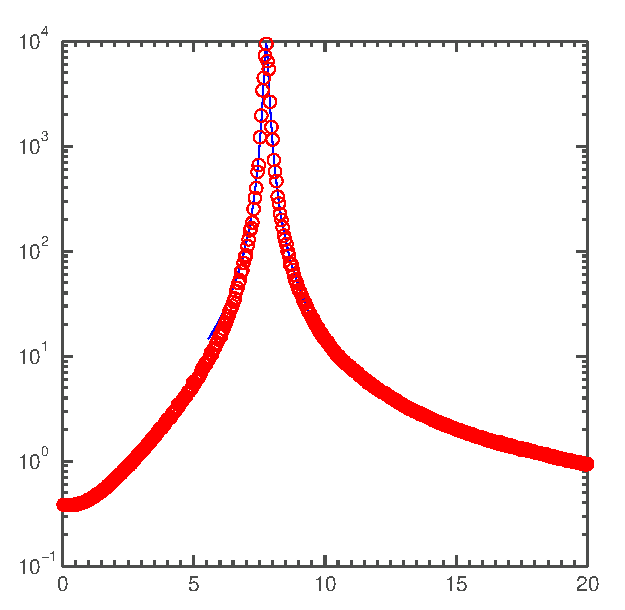
\includegraphics{sed.eps}}
\renewcommand{\figure}{Fig.}
\caption{(Colour online) Plots of the power spectrums for the selected modes as indicated by the labeled gray square markers in Fig.~\ref{fig:dispersion}(a-c). Dark blue corresponds to a superlattice without mixing, red corresponds to mixing of 80/20 and light blue corresponds to mixing of 60/40. Reported lifetimes calculated from the fitting of the Lorentzian functions (not shown) are identified by the subscripts corresponding to the color (b:dark blue, r:red, c:light blue).}
\label{fig:sed}
\end{center}
\end{figure*}
%%%

%The consequences of using same set of eigenvectors were used in the NMD procedure for mixed and non-mixed $N\times N$ is observed in Figure~\ref{fig:sed}, where for modes at low and high frequency, the peaks remain well-defined, but some intermediate frequency modes become noticeably perturbed.  
%%%
%\begin{figure}%[H]
%\begin{center}
%\scalebox{0.8}{ 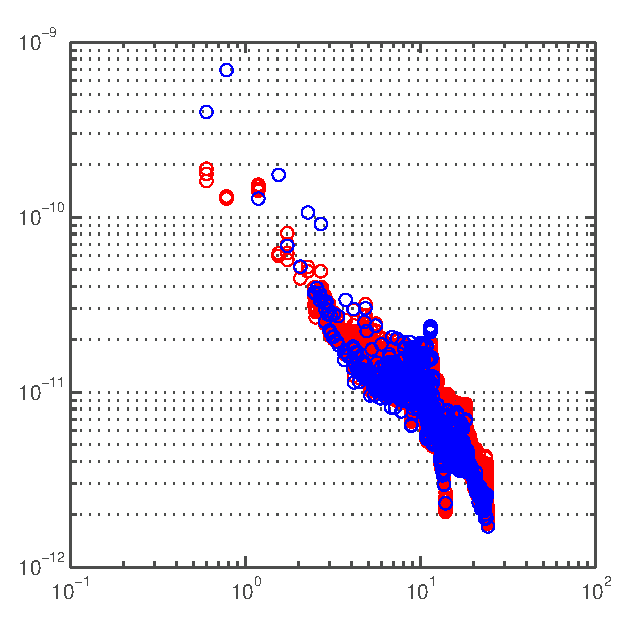
\includegraphics{/home/schuberm/Dropbox/git/plots.nogit/images/NMD_v_ALD.eps}}
%\renewcommand{\figure}{Fig.}
%\caption{Comparison between lifetimes from NMD and ALD in a $4\times4$ superlattice without interfacial mixing.}
%\label{FIG:NMD_v_ALD}
%\end{center}
%\end{figure}
%%%
%Confirm the validity of ALD

%Figure~\ref{FIG:NMD_v_ALD} shows no systematic bias between ALD and NMD for shorter lifetimes, with some systematic scatter at the longer lifetimes towards ALD. In general, ALD lifetimes are expected to be larger than NMD lifetimes because ALD neglects the contribution from $n$ order phonon processes\cite{PhysRevB.79.064301,esfarjani2011heat}, where $n$ is greater than 3.

\subsection{Lifetimes}

The phonon lifetime as a function of harmonic frequency are plotted in Fig.~\ref{FIG:lifetime}. The lifetimes for all superlattices exhibit $\omega^{-2}$ scaling at low frequencies, consistent with theoretical predictions for modes in the Debye regime associated with quadratic behaviour found in the density of states at these frequencies as seen in Fig.~\ref{fig:dispersion}(d).\cite{Klemens_Thermal_1951} For the larger period length superlattices ($8\times8$, $14\times14$), the perfect systems have two distinct scalings which terminate at the maximum frequencies of the corresponding bulk systems. As interspecies mixing is introduced, a Rayleigh scattering scaling ($\omega^{-4}$) is observed at larger frequencies for smaller superlattice period lengths ($2\times2$, $4\times4$). The $\omega^{-4}$ scaling was theoretically predicted to dominate long wavelength modes due to elastic defect scattering.\cite{PhysRev.140.A1812,klemens_scattering_1955-3, klemens_thermal_1957-2} Because the $\tau\kv$ defined by the spectral width in Eq.(\ref{EQ:lifetime}) corresponds to all possibles mechanisms of phonon interaction, the $\omega^{-4}$ scaling diverges at low frequencies and is replaced by a $\omega^{-2}$ scaling. 

There is a general downwards shift in phonon lifetimes, particularly for the higher frequency modes of short period superlattices, with some lifetimes falling below the Ioffe-Regel criterion, the limit where a mode has a lifetime less than its period of oscillation. The modes for a given superlattice have a plane wave structure, enforced by the harmonic solution of the lattice dynamics calculation. Reaching the Ioffe-Regel criterion is therefore not an indication not of spatial localization but rather of temporal localization. Modes which are below this limit can thus be considered to be non-propagating delocalized modes.\cite{allen_thermal_1993} Similar trends in the variation of lifetimes with frequency, dipping below the Ioffe-Regel criterion at intermediate frequencies and rising above at higher frequencies, have also been predicted for alloys.\cite{jason2013vc} Spatial localization has been previously invoked to explain the period-length dependence of thermal conductivity \cite{PhysRevB.61.3091} but this is not applicable to the systems studied here.
%%%
\renewcommand{\textfraction}{0.0}
\begin{figure}%[H]
\begin{center}
%\scalebox{1}{ \includegraphics{/Users/mullspace/Dropbox/git/plots.nogit/images/lifvomega.eps}}
\scalebox{1}{ \includegraphics{lifvomega.eps}}
\renewcommand{\figure}{Fig.}
\caption{Lifetimes for NMD-perfect (blue) and NMD-mixed (red). The black line corresponds to the Ioffe-Regel criterion, $2\pi\omega^{-1}$. The brown line corresponds to $\omega^{-2}$ scaling. The green line corresponds to $\omega^{-4}$ scaling. Vertical grey lines correspond to the maximum frequency observed in the bulk systems: for the lighter species, $\omega_{max}=24.7$ and for the heavier species, $\omega_{max}=14.3$. } 
\label{FIG:lifetime}
\end{center}
\end{figure}
%%%

%Fig.~\ref{FIG:lifetime} shows general agreement between the lifetimes calculated using Eq.~(\ref{EQ:tau_eff}) and lifetimes obtained from NMD under the assumption that the eigenvectors of the unmixed systems are valid for the mixed systems; both resolve the $\omega^{-2}$ scaling at low frequencies and the general smearing at intermediate and larger frequencies. At larger frequencies, Tamura theory predicts lifetimes below the Ioffe-Regel limit for all superlattice period lengths.
%%%
\begin{comment}
\begin{table}
\begin{center}
\begin{tabular*}{\textwidth}{c@{\extracolsep{\fill}}ccccc}
\hline\hline\noalign{\smallskip}
&\multicolumn{3}{c}{$N\times N$ Superlattice} \\
\cline{2-5}\noalign{\smallskip}
\hspace{1cm} & $2\times2$ & $4\times4$ & $8\times8$ & $14\times14$  \\
\noalign{\smallskip}\hline\noalign{\smallskip}
%$\tau_{eff}$   & 0.51 $\pm$ 0.51 & 0.49 $\pm$ 0.59 &  0.33 $\pm$ 0.34& 0.21 $\pm$ 0.22 \\
%ALD   & 0 $\pm$ 0 & 0.11  $\pm$  0.14 &  0.09  $\pm$  0.07 & NA \\
RMSE $\sqrt{\frac{\sum_{\pmb{\kappa}\nu}(\tau_{eff}\kv-\tau_{mixed}\kv)^2}{n}}$ &0.65 & 1.21 & 2.09 & 5.42\\
Mean $\overline{\tau_{mixed}\kv}$ &1.37 & 1.93 & 2.74 & 3.40\\
Standard Deviation $\sigma[\tau_{mixed}\kv]$ &2.34 & 2.66 & 5.53 & 11.84\\
\noalign{\smallskip}\hline\hline
\end{tabular*}
\end{center}
\renewcommand{\table}{Table.}
\caption{The root-mean-square error between Tamura theory effective lifetimes and NMD mixed lifetimes. The mean and standard deviation of the NMD mixed lifetimes are provided for context. %ALD was not used for the 14x14 case due to the computational complexity of $\Omega (N_{uc}^4)$.}
}
\label{TB:taud}
\end{table}
\end{comment}
%%%

\subsection{Thermal Conductivity}

A comparison of thermal conductivity predictions for both in-plane and cross-plane directions is presented in Tables~\ref{TB:K_CP} and~\ref{TB:K_IP}. Uncertainty in the GK prediction was found by determining the effect of removing a single molecular dynamics simulation seed upon the average estimate of thermal conductivity. Size effects were estimated by performing a convergence study. NMD predictions in both cross-plane and in-plane thermal conductivities varied by less than 10\% for systems with more than $N_x=8$ superlattice UCs along the cross-plane and $N_y=N_z=6$ UCs along the in-plane ($N_x=10$ was used for $2\times2$ superlattices to resolve the lifetime scalings). Due to the time complexity of the NMD algorithm [$O(12N_x  N_y N_z L)$], increasing the resolution of the BZ ($N_i$) was computational prohibitive. As a result of these size effects, the reported thermal conductivity predictions are presumed to carry, at a minimum, an uncertainty of 10\%.

The cross-plane and in-plane predictions from NMD and GK for perfect superlattices are in good agreement. In-plane thermal conductivity increases with increasing period length, while cross-plane thermal conductivity first decreases then increases with period length consistent with previous MD superlattice studies. \cite {PhysRevB.72.174302} In-plane thermal conductivity is nearly a factor of two larger than cross-plane thermal conductivity for all superlattices.

A thermal circuit model is presented in Table~\ref{TB:K_CP}. The boundary resistance for a perfect interface, estimated from the Direct Method ($1.4065\times10^{-8}$ [Km$^2$W$^{-1}$]), was combined with bulk thermal conductivities of the lighter material (1.2 [Wm$^{-1}$K$^{-1}$]) and the heavier material (0.7 [Wm$^{-1}$K$^{-1}$]) through their respective layer thickness, yielding an effective resistance that was inverted to obtain an effective thermal conductivity. The thermal circuit model underestimates the thermal conductivity for all superlattices, with the relative difference decreasing with increasing period length.
%No minimum in cross-plane thermal conductivity is found in the ALD predictions.
\begin{table}
\begin{center}
\begin{tabular*}{\textwidth}{c@{\extracolsep{\fill}}cccccc}
\hline\hline\noalign{\smallskip}
&&\multicolumn{4}{c}{$N\times N$ Superlattice} \\
\cline{3-6}\noalign{\smallskip}
\hspace{1cm} && $2\times2$ & $4\times4$ & $8\times8$ & $14\times14$  \\
\noalign{\smallskip}\hline\noalign{\smallskip}
\multirow{3}{*}{Perfect} &NMD & 0.29 & 0.24  & 0.32  & 0.39 \\
&GK & 0.25 $\pm$ 0.02 & 0.22 $\pm$ 0.04  &  0.29 $\pm$ 0.02  &  0.39 $\pm$ 0.03\\
%&ALD & 0.25 &	0.26  &	0.32	 &0.44\\
&Thermal Circuit & 0.07  &  0.13  &  0.23  &  0.32\\
\noalign{\smallskip}\hline
\multirow{3}{*}{Mixed} &NMD &0.19 & 0.17 & 0.28 & 0.39\\
&GK  & 0.16 $\pm$ 0.01  &  0.18 $\pm$ 0.02 &  0.29 $\pm$ 0.02 &   0.45 $\pm$ 0.06\\
&Tamura (NMD) & 0.21 & 0.15 & 0.30 & 0.37\\
%&Tamura (ALD) & 0.12 & 0.19 & 0.26 & 0.40\\
\hline\hline
\end{tabular*}
\end{center}
\renewcommand{\table}{Table.}
\caption{A comparison of the cross-plane thermal conductivity predictions [Wm$^{-1}$K$^{-1}$].}
\label{TB:K_CP}
\end{table}

\begin{table}
\begin{center}
\begin{tabular*}{\textwidth}{c@{\extracolsep{\fill}}cccccc}
\hline\hline\noalign{\smallskip}
&&\multicolumn{4}{c}{$N\times N$ Superlattice} \\
\cline{3-6}\noalign{\smallskip}
\hspace{1cm} && $2\times2$ & $4\times4$ & $8\times8$ & $14\times14$  \\
\noalign{\smallskip}\hline\noalign{\smallskip}
\multirow{2}{*}{Perfect} &NMD &0.52 & 0.51 & 0.56 & 0.60\\
&GK &0.53 $\pm$ 0.03 &  0.54 $\pm$ 0.03 &  0.61 $\pm$ 0.05  &  0.66 $\pm$ 0.07 \\
%&ALD & 0.55	& 0.53	&	0.59 	&0.63\\
\noalign{\smallskip}\hline
\multirow{3}{*}{Mixed} & NMD &0.21 & 0.25 &	0.37 & 0.47\\
&GK & 0.19 $\pm$ 0.02 &  0.30 $\pm$ 0.01  & 0.43$\pm$ 0.03 &  0.62 $\pm$ 0.07 \\   
&Tamura (NMD)& 0.22 & 0.27 & 0.38 &0.45\\
%&Tamura (ALD) & 0.17 & 0.25 & 0.34 &0.38\\
\hline\hline
\end{tabular*}
\end{center}
\renewcommand{\table}{Table.}
\caption{A comparison of the in-plane thermal conductivity predictions [Wm$^{-1}$K$^{-1}$].}
\label{TB:K_IP}
\end{table}
%%%
To provide insight into the assumption of using the perfect eigenvectors for the mixed superlattices as described in Sec.~\ref{SEC:methods}, we use Tamura elastic mass defect scattering theory \cite{tamura_isotope_1983} to modify the lifetimes predicted for perfect superlattices [$\tau_{perfect}\kv$] through the Matthiesen rule %as done by Luckyanova et al. \cite{Luckyanova16112012} 
%%%
\begin{equation}\label{EQ:tau_eff}
\begin{split}
\frac{1}{\tau_{effective}\kv} = \frac{1}{\tau_{defect}\kv}+\frac{1}{\tau_{perfect}\kv} ,
\end{split}
\end{equation}
%%%
where
%%%
\begin{equation}\label{EQ:tau_d}
\begin{split}
\frac{1}{\tau_{defect}\kv} = \frac{\pi}{2N_{uc}}\omega^2\kv 
\sum_{\pmb{\kappa'},\nu'} \delta\left[ \omega\kv - \omega\kvp \right]\sum_{b} g_2(b) 
|e^*\kvbap \cdot e\kvba |^2 ,
\end{split}
\end{equation}
%%%
$N_{uc}$ is the total number of unit cells considered, and $g_2(b)$ is the coupling term which defines the strength of the mass disordering
%%%
\begin{equation}\label{EQ:g(b)}
\begin{split}
g_2(b) = \sum_\mu c_{\mu}(b)\left[1-\frac{m_{\mu}(b)}{\overline{m(b)}}\right]^2, 
\end{split}
\end{equation}
%%%
where $c_\mu(b)$ is the concentration of the mixing, $m_\mu(b)$ is the mass of the $\mu$-th species and $\overline{m(b)}$ is the average mass for the $b$ atom in the unit cell. Given that there are two atom types in the superlattice unit cell, the lighter atom can be considered to be a mass defect of the heavier portion of the superlattice, with the reverse being equally true. $g_2(b)$ was set to be zero if atom $b$ was unmixed (for atoms that do not reside within one monolayer of the interface). The delta function in Eq.~(\ref{EQ:tau_d}) is broadened into a Lorentzian function with width on the order of the frequency level spacing imposed by the finite size of the systems.\cite{allen_thermal_1993}

For short period mixed superlattices, the in-plane and cross-plane predictions are reduced from their corresponding perfect system and approach the alloy limit (0.21- 0.28 [Wm$^{-1}$K$^{-1}$]), with the mixed $2\times 2$ losing much of its anisotropy between the in-plane and cross-plane directions. From Table~\ref{TB:K_CP}, the predictions for mixed superlattices from NMD (using perfect eigenvectors), Tamura theory and GK are in good agreement. From Table~\ref{TB:K_IP}, for mixed superlattices, NMD and Tamura theory, while in good agreement respectively,  predict a lower in-plane thermal conductivity, with the systematic difference increasing with period length. This is indicative of the disruption of the superlattice phonon modes through interfacial mixing which are expected to contribute to thermal transport. With increasing period length, these modified modes are more likely to be represented by the modes found in bulk systems and may explain the discrepancy between NMD or Tamura theory and GK.

%%%
\begin{comment}
\begin{table}
\begin{center}
\begin{tabular}{lcc}
\hline\hline\noalign{\smallskip}
&\multicolumn{2}{c}{Method} \\
\cline{2-3}\noalign{\smallskip}
$k$ & NMD  & GK  \\
\noalign{\smallskip}\hline\noalign{\smallskip}
Cross-Plane Perfect  & 0.24 $\pm$ 0.02 & 0.22 $\pm$ 0.04\\
Cross-Plane 80/20    & 0.17  $\pm$ 0.01   &   0.18 $\pm$ 0.02 \\
Cross-Plane 60/40    & 0.18  $\pm$ 0.01   &   0.19 $\pm$ 0.02 \\
In-Plane Perfect   & 0.52 $\pm$ 0.03 & 0.54 $\pm$ 0.03  \\
In-Plane 80/20  & 0.25 $\pm$ 0.02 & 0.30 $\pm$ 0.01  \\
In-Plane 60/40   & 0.20 $\pm$ 0.02 & 0.26 $\pm$ 0.01  \\
\noalign{\smallskip}\hline\hline
\end{tabular}
\end{center}
\renewcommand{\table}{Table.}
\caption{A comparison of the thermal conductivity predictions [$Wm^{-1}K^{-1}$] predictions for a $4\times4$ superlattice.}
\label{TB:validate}
\end{table}
\end{comment}
%%%

From Fig.~\ref{FIG:MFP_cp}, there is a clear reduction in the contribution to cross-plane thermal conductivity in perfect superlattices from modes with a MFP greater than the period length as period length increases. This trend is consistent with the theoretical predictions from Mahan that a minimum thermal conductivity occurs as the transport behaviour shifts from a wave-regime to particle-regime.\cite{PhysRevLett.84.927,PhysRevB.56.10754} This same trend is observed in the contribution curves for the in-plane conductivity (not shown). The minimum cross-plane thermal conductivity in the for perfect superlattices occurs at a point where the average MFP is slightly greater than the period length between $4 \times 4$ and $8 \times 8$. This minimum disappears for the mixed superlattices.

The dimensional value of the peak MFP in perfect superlattices, for both in-plane and cross-plane, does not vary significantly as a function of period length. For short period superlattices ($2\times2$, $4\times4$ and $8\times8$), interfacial mixing shifts the average MFP towards the period length and reduces its respective contribution, indicative of the transition of thermal transport from superlattice phonons to thermal transport from phonons which may or may not map to those belonging to the perfect dispersion. This trend further supports the fact that superlattice phonons become disrupted by interfacial mixing, thereby diminishing the enhancing effects of the secondary periodicity upon cross-plane thermal conductivity. At large enough period lengths, the effect of interspecies mixing has a negligible effect on phonon MFP, as the corresponding lifetimes are less affected with increasing period length (Fig.~\ref{FIG:lifetime}) because of the decrease in the number of interfaces per unit of volume. \cite{PhysRevB.79.075316}
%%%
\begin{figure}%[H]
\begin{center}
\scalebox{1}{ \includegraphics{MFP_cp.eps}}
\renewcommand{\figure}{Fig.}
\caption{Phonon mean free path normalized by the period length contribution to the cross-plane thermal conductivity. From top to bottom $2\times2$, $4\times4$, $8\times8$ and $14\times14$ superlattices. Color corresponds to those used in Fig.~\ref{FIG:lifetime}. Average MFP is reported; subscripts correspond to the color of marker [b:blue (perfect), r:red (mixed)]. Orange corresponds to lighter bulk and green corresponds to heavier bulk.}
\label{FIG:MFP_cp}
\end{center}
\end{figure}
%%%

The sharp discontinuities in the contribution distribution at longer MFPs is consequence of the limited resolution of the BZ enforced by the MD domain. This has been observed in other mode by mode analysis techniques, such as the real space force constant extraction from DFT method used by Esfarjani, where the limited resolution manifested in a stepwise behavior of thermal conductivity accumulation function of bulk silicon. \cite{PhysRevB.84.085204} The linear behavior of the dispersion near the gamma point of the BZ and the $\omega^{-2}$ scaling of the lifetimes allowed for the contribution of these unresolved long-wavelength modes to be estimated. The linear extrapolation procedure used to predict bulk thermal conductivities \cite{PhysRevB.81.214305} was not used in previous superlattice studies \cite{doi:10.1021/nl202186y,Luckyanova16112012} and is not used here. The complicated dispersion [Fig.~\ref{fig:dispersion}(a-c)] does not guarantee that such an approach is viable, as such, understanding size effects in superlattices warrants further work.

\section{Superlattice phonons}

Past literature has cited superlattices as a structure where coherent effects upon thermal transport are possible; the trend in thermal conductivity as a function of period length being used to justify such a claim.\cite{PhysRevB.67.195311,PhysRevB.72.174302,PhysRevB.61.3091} Here we have reproduced comparable trends simply by adopting the correct phonon dispersion for our analysis, implying an equivalency between a dispersion effect and a coherence effect. By using molecular dynamics, we do not impose any restrictions upon phonon dynamics but let the system move through phase space naturally and thus should sufficiently capture all classical effects. 

The reasons are twofold for the ambiguity attached to the term \textit {coherent effects}: its association with exotic configurations of material, like porous silicon \cite{doi:10.1021/nl102918q} where the secondary periodicity emerges from the introduction of the repeated holes or between nanoparticles in a nanofluidic system \cite{Keblinski2002855} and from previous experimental coherent phonon studies \cite{PhysRevLett.73.740,PhysRevB.75.195309} that do not focus upon thermal transport. Coherent effects, for that matter, are found in bulk systems since coherence requires the constructive or destructive interference of waves.

One measure of coherent effects is coherence length, defined as the distance a plane wave travels until its phase becomes randomized and thus only applies in the wave picture of phonon transport. Although there does not appear to be a formal equation for phonon coherence length,\cite{chen2005nanoscale} adopting a unit cell that spans a single superlattice period to generate the modified dispersion relation allows one to ignore the difference between the MFP and coherence length.\cite{PhysRevB.67.195311} In this context, the MFPs greater than the period length cannot be interpreted any differently than MFPs greater than the lattice constant of a bulk crystalline structure. This is confirmed by observing that MFP contribution distribution, normalized by the superlattice period length, for the lighter (orange) and heavier (green) bulk systems [Fig.~\ref{FIG:MFP_cp}] follows the MFP distribution for the perfect superlattices. Mixing shifts the MFP distribution downward; evidence that roughness and disorder, in general, destroy coherent effects.\cite{PhysRevB.67.195311,dames_682} The successful application of Tamura's elastic defect scattering theory to systems studied here is consistent with Pomeranchuk's argument that inelastic defect scattering has negligible effects upon thermal transport.\cite{pomeranchuk1942thermal} 
%Phase is assumed to be randomized through inelastic phonon-phonon, but not elastic boundary or impurity scattering \cite{chen2005nanoscale}. Furthermore, the inability for NMD and ALD to estimate the in-plane thermal conductivity in mixed superlattices indicates the disruption of the superlattice dispersion. 

Finally, by relying upon the BTE, any coherent effect is abstracted into the phonon-as-a-particle interpretation. Thus, we believe, coherent effects or equivalently, dispersion effects, are of consequence when one cannot use the bulk material phonon properties as particles to predict thermal transport in a non-bulk system. This is clearly the case for all the systems studied here, including the larger period superlattices ($8 \times 8$ and $14 \times 14$), as evidenced by the discrepancy between the bulk-based thermal circuit model predictions and the NMD and GK predictions [see Table~\ref{TB:K_CP}].

\section{Summary}

We show the reduction in the contribution to cross-plane thermal conductivity from MFPs greater than the superlattice period as the period length is increased, for both perfect and mixed. Differences between in-plane and cross-plane components of group velocity are responsible for the respective differences between thermal conductivity [Fig.~\ref{fig:dispersion}(a-c)]. Debye scaling at low frequency modes in perfect and mixed superlattices and Raleigh scattering at intermediate frequencies in mixed superlattices in observed (Fig.~\ref{FIG:lifetime}). Interspecies mixing reduces phonon lifetimes thereby shifting the phonon MFP spectrum downward (Fig.~\ref{FIG:MFP_cp}) and disrupts superlattice phonon transport (Fig.~\ref{fig:sed}(B) and Table~\ref{TB:K_IP}), thus reducing in-plane and cross-plane thermal conductivity.

\newpage
\bibliographystyle{apsrev}
\bibliography{superlattice.bib}

\end{document}

